% Preamble
\documentclass[a4paper, 12pt]{article}
\usepackage[margin=1in]{geometry} % Set margin
\usepackage{pdfpages} % Insert pdf pages
\usepackage{amssymb,amsmath,amsthm, amsfonts} % Math libraries

% Custom commands
\newcommand{\sub}[1]{\subsection{\underline{#1}}}
\newcommand{\subsub}[1]{\subsubsection{\underline{#1}}}
\newcommand{\R}{\ensuremath{\mathbb{R}}}
\newcommand{\F}{\ensuremath{\mathbb{F}}}
\newcommand{\N}{\ensuremath{\mathbb{N}}}
\newcommand{\Onef}{\ensuremath{1_{\F}}}
\newcommand{\Zerof}{\ensuremath{0_{\F}}}
\newcommand{\eqbcuz}[1]{\text{~$\stackrel{(#1)}{=}$~}}
\newcommand{\eq}[1]{\begin{align*}#1\end{align*}}
\newcommand{\eqn}[1]{\begin{align}#1\end{align}}
\newcommand{\set}[1]{\big{\{} #1 \big{\}}}
\renewcommand{\qed}{\hfill\(\qedsymbol\)}
\newtheorem{lemma}{Lemma}

% Begin Document %
\begin{document}

% Title Page
\begin{titlepage}
    %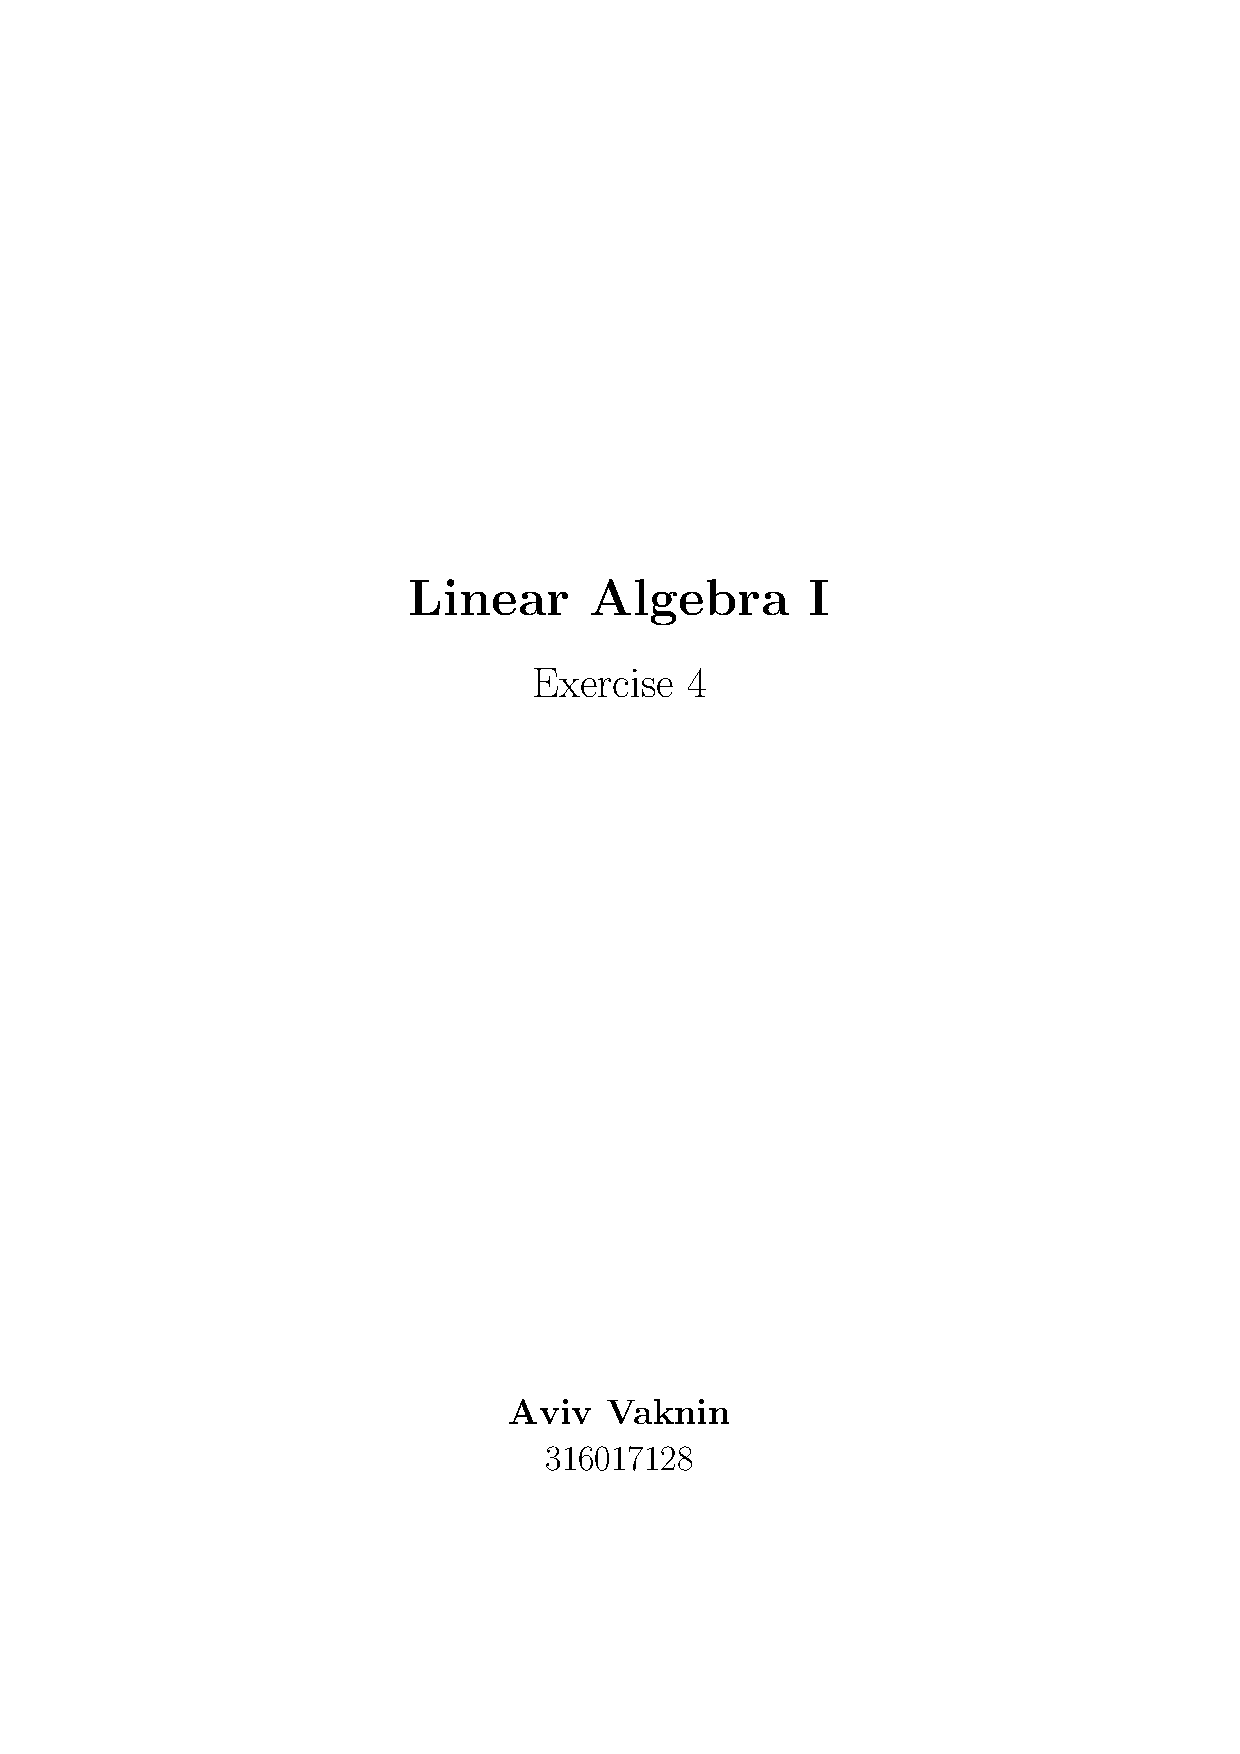
\includepdf{title.pdf}
\end{titlepage}

% 3
\setcounter{section}{2}
\section{Calculate \textit{AC}, \textit{BC}, \textit{ABC} and \textit{BAC}}
\eq{
    AC=\begin{bmatrix}
        c^1_1 & c^1_2 & c^1_3 \\
        c^3_1 & c^3_2 & c^3_3 \\
        c^2_1 & c^2_2 & c^2_3
    \end{bmatrix}
    \\
    BC=\begin{bmatrix}
        c^3_1 & c^3_2 & c^3_3 \\
        c^1_1 & c^1_2 & c^1_3 \\
        c^2_1 & c^2_2 & c^2_3
    \end{bmatrix}
    \\
    A(BC)=\begin{bmatrix}
        c^3_1 & c^3_2 & c^3_3 \\
        c^2_1 & c^2_2 & c^2_3 \\
        c^1_1 & c^1_2 & c^1_3
    \end{bmatrix}
    \\
    B(AC)=\begin{bmatrix}
        c^2_1 & c^2_2 & c^2_3 \\
        c^1_1 & c^1_2 & c^1_3 \\
        c^3_1 & c^3_2 & c^3_3
    \end{bmatrix}
}

% 6
\setcounter{section}{5}
\section{Prove that \eq{A(\lambda{B})=B(\lambda{A})=\lambda(AB)}}
We'll prove this by showing:
\eq{
    [A(\lambda{B})]^i_j=[B(A\lambda)]^i_j=[\lambda(AB)]^i_j
}
Therefore, if for all of the matrices, all of the cells are identical, the matrices are the same.
\eq{
    &[A(\lambda{B})]^i_j=\sum^n_{k=1}a^i_k(b^k_j\lambda)\\
    &[B(A\lambda)]^i_j=\sum^n_{k=1}b^k_j(a^i_k\lambda)\\
    &[\lambda(AB)]^i_j=\lambda(\sum^n_{k=1}a^i_kb^k_j)
}
As all of the operations are happening inside $\F$, we can factor the $\lambda$, and therefore:
\eq{
    &[A(\lambda{B})]^i_j=\sum^n_{k=1}a^i_k(b^k_j\lambda)=\lambda(\sum^n_{k=1}a^i_kb^k_j)\\
    &[B(A\lambda)]^i_j=\sum^n_{k=1}b^k_j(a^i_k\lambda)=\lambda(\sum^n_{k=1}a^i_kb^k_j)
}
Therefore, we've shown that:
\eq{
    [A(\lambda{B})]^i_j=[B(A\lambda)]^i_j=[\lambda(AB)]^i_j
}
And therefore:
\eq{
    A(\lambda{B})=B(\lambda{A})=\lambda(AB)
}
\qed

% 7
\section{Prove that \eq{A(\lambda{C}+D)=O}}
According to question \textbf{5}:
\eq{
    A(\lambda{C}+D)=A\lambda{C}+AD
}
According to question \textbf{6}:
\eq{
    A\lambda{C}+AD=\lambda\cdot{AC}+AD
}
It is given that $AC=AD=O$, therefore:
\eq{
    \lambda\cdot{AC}+AD=\lambda\cdot{O}+O
}
According to the properties of matrix scalar multiplication:
\eq{
    a\cdot{O}=O
}
Therefore:
\eq{
    \lambda\cdot{O}+O=O+O=O
}
\qed

% 10
\setcounter{section}{9}
\section{}

% End Document %
\end{document}